\documentclass[a4paper, 12pt]{article}
\usepackage[slovene]{babel}
\usepackage[utf8]{inputenc}
\usepackage[T1]{fontenc}
\usepackage{mathtools}
\usepackage{amsmath}
\usepackage{tikz}
\usepackage{pgfplots}
\usepackage{hyperref}

\setlength{\parindent}{0px}
\setlength{\parskip}{10px}

\begin{document}

\begin{figure}[h!]
	\centering
	\caption{3D funkcija}
	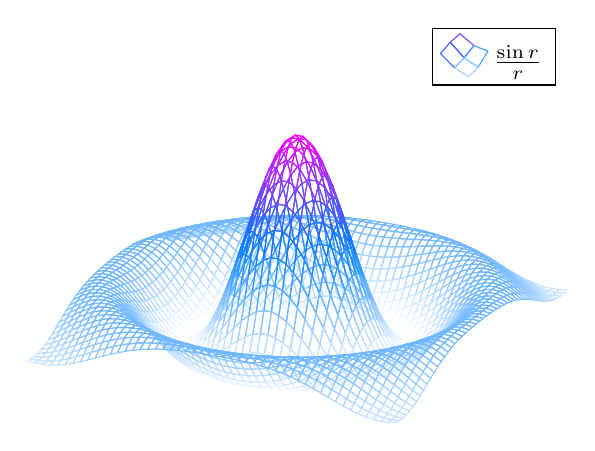
\begin{tikzpicture}
	\begin{axis}[
	hide axis,
	colormap/cool,
	]
	\addplot3[
		mesh,
		samples=50,
		domain=-8:8,
	]
	{sin(deg(sqrt(x^2+y^2)))/sqrt(x^2+y^2)};
	\legend{$\frac{\sin r}{r}$}
	\end{axis}
	\end{tikzpicture}
\end{figure}

\begin{figure}[h!]
	\centering
	\caption{3D funkcija}
	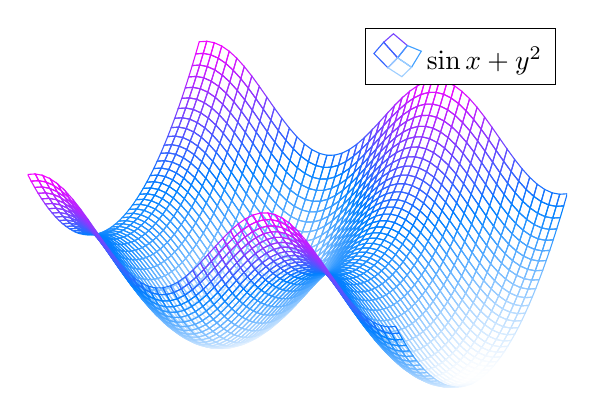
\begin{tikzpicture}
	\begin{axis}[
	hide axis,
	colormap/cool,
	]
	\addplot3[
		mesh,
		samples=50,
		domain=-5:5,
	]
	{10*sin(deg(x)) + y*y};
	\legend{$\sin x + y^2$}
	\end{axis}
	\end{tikzpicture}
\end{figure}

\end{document}
